\chapter{Uploading Facebook Reels for Reach}

This chapter records a School of Hard Knocks tutorial on uploading a Facebook Reel and packaging it for reach. The lecture is practical rather than theoretical: Josh does not derive a ranking model, but he does give a sequence of choices that can be repeated. We will keep that sequence intact and treat the few equations below as bookkeeping devices, not as claims about Facebook's internal algorithm. The source is a School of Hard Knocks demonstration curated by LazyingArt LLC with Video2Book.

\section{The Problem: Publish the Reel and Improve Its Reach}

Josh opens with a narrow promise. We are going to upload a Facebook Reel and try to get the maximum exposure from it. The point is not to study every feature of Facebook. The point is to walk through the upload path and notice where the creator can make deliberate choices.

A useful way to preserve the lecture's order is to write the workflow as an ordered tuple:
\begin{equation}
\mathcal{W}
=
(P,\ R,\ V,\ S,\ C,\ D,\ H,\ \mathrm{Share}).
\end{equation}
Here \(P\) is the page, \(R\) is the Reel creation path, \(V\) is the selected video, \(S\) is the added sound layer, \(C\) is the cover, \(D\) is the description, and \(H\) is the hashtag set. This notation is deliberately modest. It simply keeps the process from collapsing into the vague instruction ``post a Reel.''

The first transition in the lecture is from introduction to screen recording. Before Josh begins clicking through the process, he removes one practical obstacle: he says the mobile and desktop processes are effectively the same, though he will demonstrate on the mobile app. That lets us follow one concrete interface without treating it as a separate mobile-only method.

\section{Page, Reel, and Video Asset}

The first operational choice is the publishing identity. We do not upload the video into an abstract feed; we choose the page that will carry the post. In the lecture that page is School of Hard Knocks. The sequence is: log in, go to pages, select the page, find the place to create a post, and choose to create a Reel.

Once the Reel path is open, Josh selects the video asset. The clip he chooses is described as asking a social media expert and influencer for advice. At this point the core content has been chosen, and the rest of the lecture concerns the package around that content.

\begin{definition}
The \emph{Reel package} is the video together with the surrounding choices that prepare it for discovery and action:
\begin{equation}
\mathrm{Reel\ package}
=
\mathrm{video}
+
\mathrm{sound\ layer}
+
\mathrm{cover}
+
\mathrm{description}
+
\mathrm{hashtags}.
\end{equation}
\end{definition}

This is not a formal equation about reach. It is a way to separate the asset from its presentation. The same video can be posted with different sounds, covers, descriptions, and hashtags; the lecture is about making those choices consciously.

\begin{figure}
\centering
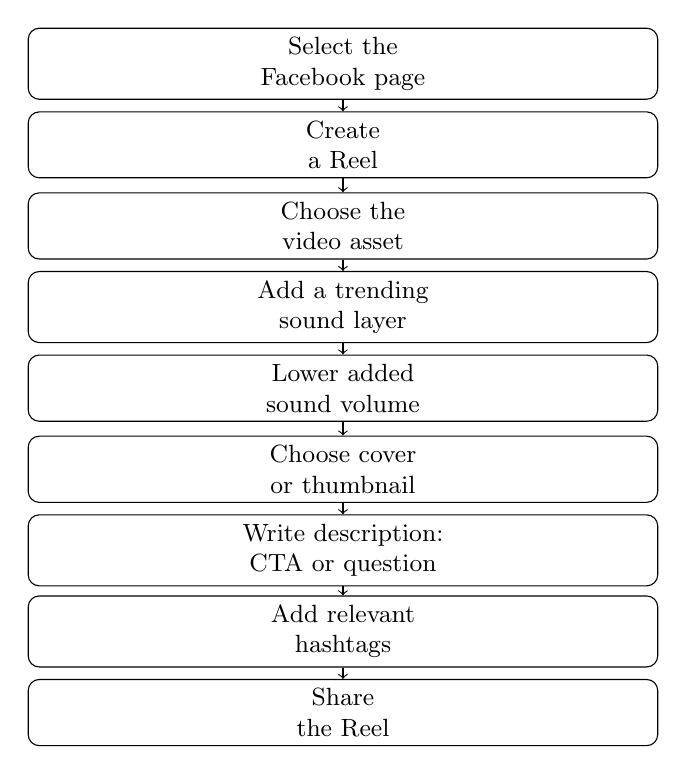
\begin{tikzpicture}[
  box/.style={draw, rounded corners, align=center, text width=0.64\linewidth, minimum height=0.58cm},
  every node/.style={font=\small}
]
\node[box] (p) at (0,0) {Select the\\Facebook page};
\node[box] (r) at (0,-1.03) {Create\\a Reel};
\node[box] (v) at (0,-2.06) {Choose the\\video asset};
\node[box] (s) at (0,-3.09) {Add a trending\\sound layer};
\node[box] (m) at (0,-4.12) {Lower added\\sound volume};
\node[box] (c) at (0,-5.15) {Choose cover\\or thumbnail};
\node[box] (d) at (0,-6.18) {Write description:\\CTA or question};
\node[box] (h) at (0,-7.21) {Add relevant\\hashtags};
\node[box] (x) at (0,-8.24) {Share\\the Reel};
\draw[->] (p) -- (r);
\draw[->] (r) -- (v);
\draw[->] (v) -- (s);
\draw[->] (s) -- (m);
\draw[->] (m) -- (c);
\draw[->] (c) -- (d);
\draw[->] (d) -- (h);
\draw[->] (h) -- (x);
\end{tikzpicture}
\caption{A compact reconstruction of the spoken workflow. The diagram is transcript-derived rather than a visible board diagram.}
\end{figure}

\section{The Sound Layer as an Exposure Lever}

After the video is selected, Josh introduces the first tactical claim. He says that, in his experience from TikTok and content creation, adding a sound tends to get videos more exposure. He then chooses a trending sound or artist; the example named in the transcript is ``Whoa'' by Lil Baby.

We should preserve both parts of the claim: the action and its evidentiary status. In informal notation, let \(E\) stand for exposure and let \(S\) stand for the presence of an added sound layer. The lecture supports only the directional, experiential statement
\begin{equation}
\Delta E(S) > 0
\qquad
\text{in Josh's reported experience.}
\end{equation}
This should not be read as a measured law of the platform. It is a creator's operating rule: add a sound because, in his experience, it has helped distribution.

\subsection{Question \& Answer}

\paragraph{Question.}
Why add music if we do not actually want the audience to hear that music?

\paragraph{Answer.}
Josh separates the platform signal from the audible experience. He attaches the trending sound, but then lowers its volume so the original clip remains the main audio. If \(A_0\) denotes the original video audio and \(A_{\mathrm{trend}}\) denotes the added sound, the tactic can be written as the update
\begin{align}
v_{\mathrm{trend}} &\longleftarrow \epsilon v_{\mathrm{trend}},
\qquad 0<\epsilon\ll 1, \\
A_{\mathrm{heard}} &= A_0 + \epsilon A_{\mathrm{trend}}, \\
\mathrm{package} &\text{ still contains the trending sound layer.}
\end{align}
The notation is ours, but the distinction is Josh's: keep the sound attached to the Reel while preventing it from overpowering the original content.

\section{Cover and Composer}

After the sound step, Josh moves toward the cover or thumbnail. The transcript is slightly uneven around this transition, but the reliable sequence is that he sets the cover and then moves into the New Reel composer. The next stage is no longer choosing the video content; it is deciding how the video will be presented at posting time.

\begin{figure}
\centering

\includegraphics[width=0.62\linewidth]{lecture_177_figure_02.png}
\caption{The Facebook New Reel composer, with the description field open and Public visibility selected.}
\end{figure}

The screenshot is important because it shows the place in the interface where the next spoken recommendation applies. The visible field says ``Write a description...''; the visibility panel asks who can see the Reel; ``Public'' is selected; and the keyboard is open. The screenshot does not show the completed call-to-action text. It shows the entry point for that text.

\section{Description, Action, and Experimentation}

Josh's next move is to the description. He says he likes to add either a call to action or a thought-provoking question to get people to watch the full video or follow for more content. In this example he leans toward a call to action: ask people to follow for more content like this.

We can write the description choice as
\begin{equation}
D \in
\{\mathrm{call\ to\ action},\ \mathrm{thought\ provoking\ question}\}.
\end{equation}
The important part is not that this set is exhaustive. It is that Josh treats the description as a conversion surface. The video catches attention; the description can ask for a next action.

He then immediately softens any temptation to turn one phrase into a formula. The advice is to experiment with different phrases, questions, and calls to action, and then observe what gets traction. A cautious way to record that testing loop is
\begin{equation}
D_{n+1}
=
\mathrm{adjust}(D_n;\ \mathrm{observed\ traction}),
\end{equation}
where \(D_n\) is the current description style. This is not a platform model. It is a practical iteration rule: try, observe, adjust.

\section{Hashtags and Niche Relevance}

After the call to action, Josh adds hashtags. His rule has two layers of relevance. Some hashtags should match the particular post, such as social media or influencer for the selected clip. Others should match the broader page niche, such as business, entrepreneur, or finance for School of Hard Knocks.

The one numerical guideline in the lecture is his usual hashtag count:
\begin{equation}
H \approx 6\text{--}7.
\end{equation}
Here \(H\) denotes the number of hashtags Josh says he typically uses. This is a reported practice, not a proven optimum.

The description and hashtag layers therefore do different jobs:
\begin{align}
D &: \text{turn attention into an action or continued watching}, \\
H &: \text{mark topic relevance and page-niche relevance}.
\end{align}
This separation is useful. It keeps us from treating every piece of text around the Reel as if it served the same purpose.

\section{Share and Strategic Placement}

The final mechanical step is to share the Reel. Once the upload is complete, Josh shifts from the narrow tutorial to the broader brand frame. Facebook Reels are not presented as the whole strategy. They are one part of a larger effort to build awareness around a brand across social channels.

A concise reconstruction of that closing idea is
\begin{equation}
\mathrm{brand\ awareness}
\leftarrow
\mathrm{consistent\ publishing\ across\ social\ channels}.
\end{equation}
This is a summary of the strategic direction, not a measured causal formula. The lecture's practical message is that posting the Reel is an execution step, while the reason for doing it is broader: repeated visibility around the brand.

\section{Summary}

The lecture unfolds as a repeatable path: select the page, create the Reel, choose the video, add a trending sound, lower that sound's volume, choose a cover, write a description, add relevant hashtags, and share. The visual frame of the New Reel composer anchors the description stage, where the call to action would be entered and the public visibility setting is visible.

The strongest lesson is the separation of roles. The video carries the content. The sound layer may help discovery, according to Josh's experience. The cover frames the preview. The description asks for action or continued attention. The hashtags connect the post to both its topic and its niche. The chapter should keep those claims source-conscious: useful as creator practice, but not presented as a guaranteed model of platform behavior.